%%%%%%%%%%%%%%%%%%%%%%%%%%%%%%%%%%%%%%%%%%%%%%%%%%%%%%%%%%%%%%%%%%%%%%%%%%%%%%%%
%2345678901234567890123456789012345678901234567890123456789012345678901234567890
%        1         2         3         4         5         6         7         8

\documentclass[letterpaper, 10 pt, conference]{ieeeconf}  % Comment this line out if you need a4paper

%\documentclass[a4paper, 10pt, conference]{ieeeconf}      % Use this line for a4 paper

\IEEEoverridecommandlockouts                              % This command is only needed if 
                                                          % you want to use the \thanks command

\overrideIEEEmargins                                      % Needed to meet printer requirements.

\usepackage{lmodern}
\usepackage{textcomp}
\usepackage{amsmath}
\usepackage{lipsum}

\usepackage{graphicx}
\graphicspath{ {img/} }

\newcommand{\norm}[1]{\left\lVert#1\right\rVert}


\title{
\LaTeX\ is an enjoyable way to write scientific papers
}


\author{Gudjon Einar Magnusson$^{1}$
\thanks{$^{1}$Gudjon Einar Magnusson is a graduate student in the department of computer science,
        University of Maryland, College Park
        {\tt\small gmagnusson@fc-md.umd.edu}}%
}


\begin{document}



\maketitle
\thispagestyle{empty}
\pagestyle{empty}


%%%%%%%%%%%%%%%%%%%%%%%%%%%%%%%%%%%%%%%%%%%%%%%%%%%%%%%%%%%%%%%%%%%%%%%%%%%%%%%%
\begin{abstract}

In this short paper I will show that \LaTeX\ is much more enjoyable way to write scientific papers than
using primitive text editors such as Microsoft Word\texttrademark\

\end{abstract}


%%%%%%%%%%%%%%%%%%%%%%%%%%%%%%%%%%%%%%%%%%%%%%%%%%%%%%%%%%%%%%%%%%%%%%%%%%%%%%%%
\section{INTRODUCTION}

This paper contains no information, but I want it to look good so I'm going to add a lot of text. The main point is that latex is better than word\cite{web:kent} and I will explain why in section \ref{fig} and section \ref{eq}.

\lipsum[1]


\label{fig}
\section{FIGURES}

With latex it's easy to add figures and add references to them in the text. In figure \ref{fig:baxter} we see Baxter and in figure \ref{fig:atlas} we see Atlas. Just drop in the image, give them a name and latex automatically handles the numbering and cross referencing. Unlike the cross reference in Word that break all the time. You don't really know where on the page the image will end up, but who cares.

\begin{figure}[h]
\centering
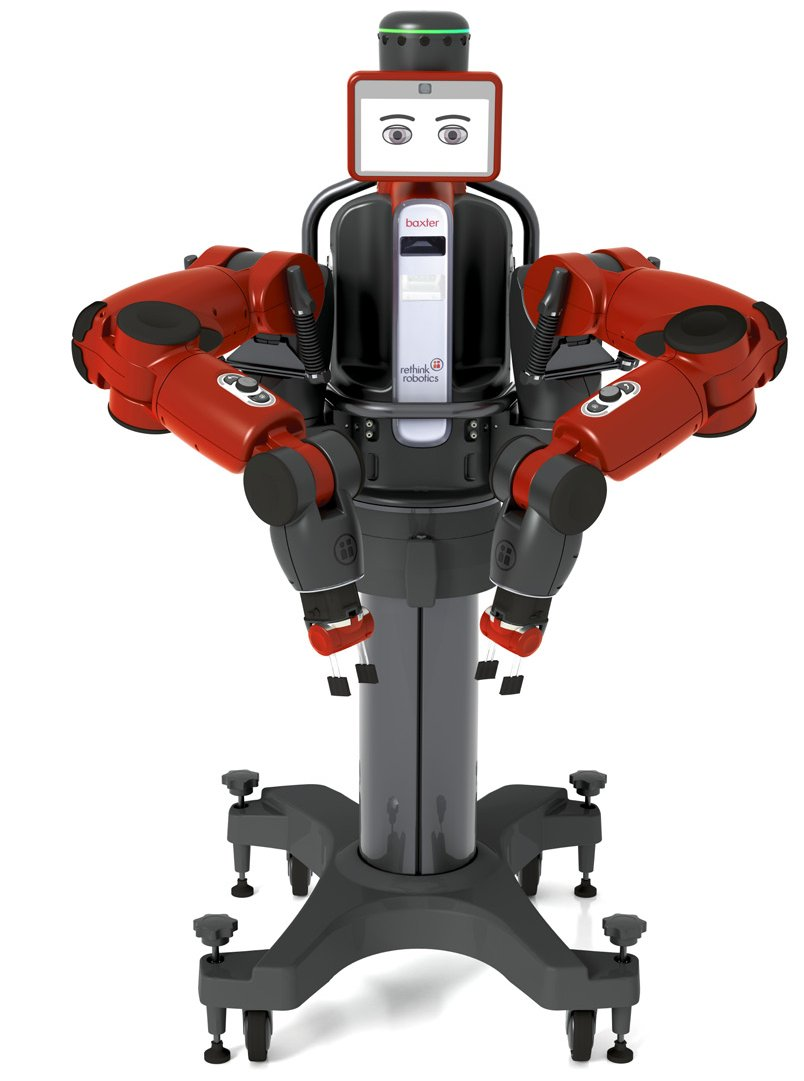
\includegraphics[width=0.25\textwidth]{baxter}
\caption{This is Baxter, the friendly robot helper from Rethink Robotics}
\label{fig:baxter}
\end{figure}

\begin{figure}[h]
\centering
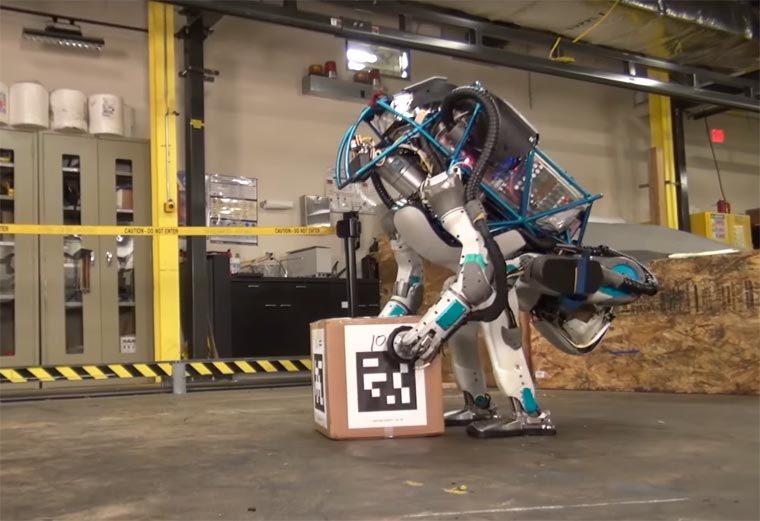
\includegraphics[width=0.25\textwidth]{atlas}
\caption{This is Atlas, the slightly scary looking but incredibly impressive humanoid robot from Boston Dynamics}
\label{fig:atlas}
\end{figure}

\label{eq}
\section{EQUATIONS}

The best part of writing in latex is playing with equations. You can add stand alone equations and reference them in the text. For example, I like to talk about equation \ref{eq:sumSq}, the sum of square differences.

\begin{equation} \label{eq:sumSq}
\sum_{i=1}^{N} \norm{x_i - y_i} ^{2}
\end{equation}

Yous can also drop math right into your text, like so $\frac{\alpha - \beta}{2}$ or whatever\cite{web:texMath}.

\section{CONCLUSIONS}

I expect that you have learned absolutely nothing from reading this nonsense, but it looks good right.

Also, don't walk around in the woods by your self\cite{book:lrr}

\addtolength{\textheight}{-12cm}   % This command serves to balance the column lengths
                                  % on the last page of the document manually. It shortens
                                  % the textheight of the last page by a suitable amount.
                                  % This command does not take effect until the next page
                                  % so it should come on the page before the last. Make
                                  % sure that you do not shorten the textheight too much.

%%%%%%%%%%%%%%%%%%%%%%%%%%%%%%%%%%%%%%%%%%%%%%%%%%%%%%%%%%%%%%%%%%%%%%%%%%%%%%%%


\bibliography{ref}
\bibliographystyle{ieeetr}

\end{document}
